In general, our architecture is capable of learning meaningful and reliable measures of uncertainty in its forecasts\added{, and our forecasts outperform the basic benchmark of persistence forecasting}. We \replaced{focus in our discussion on the}{discuss the architecture} performance \replaced{of the}{here by restricting ourselves to} six-hour ahead probabilistic forecasts \deleted{from the network trained with both L1 and solar disk inputs} \replaced{because this forecast window is long enough that information from the L1 point is insufficient to forecast storm arrivals, allowing us to evaluate whether our network is able to leverage information from the solar disk.}{for three different storms: two caused by CMEs (Figure 2A & B) and one resulting from a co-rotating interaction region (CIR) (Figure 2C). One to six hour ahead forecasts, as well as detailed comparison of the networks trained with only L1 data and both L1 and solar disk inputs, can be found in the Supplement.}  

% storm exmaples
\subsection{\added{Storm Case Studies}}
\added{We present and discuss in this section six hour ahead forecasts} for three different storms: two caused by CMEs (Figure~\ref{fig:storms}A \& B) and one resulting from a co-rotating interaction region (CIR) (Figure~\ref{fig:storms}C). One to six hour ahead forecasts, as well as detailed comparison of the networks trained with only L1 data and both L1 and solar disk inputs, can be found in the Supplement.

\begin{figure}[htbp]
  \centering
  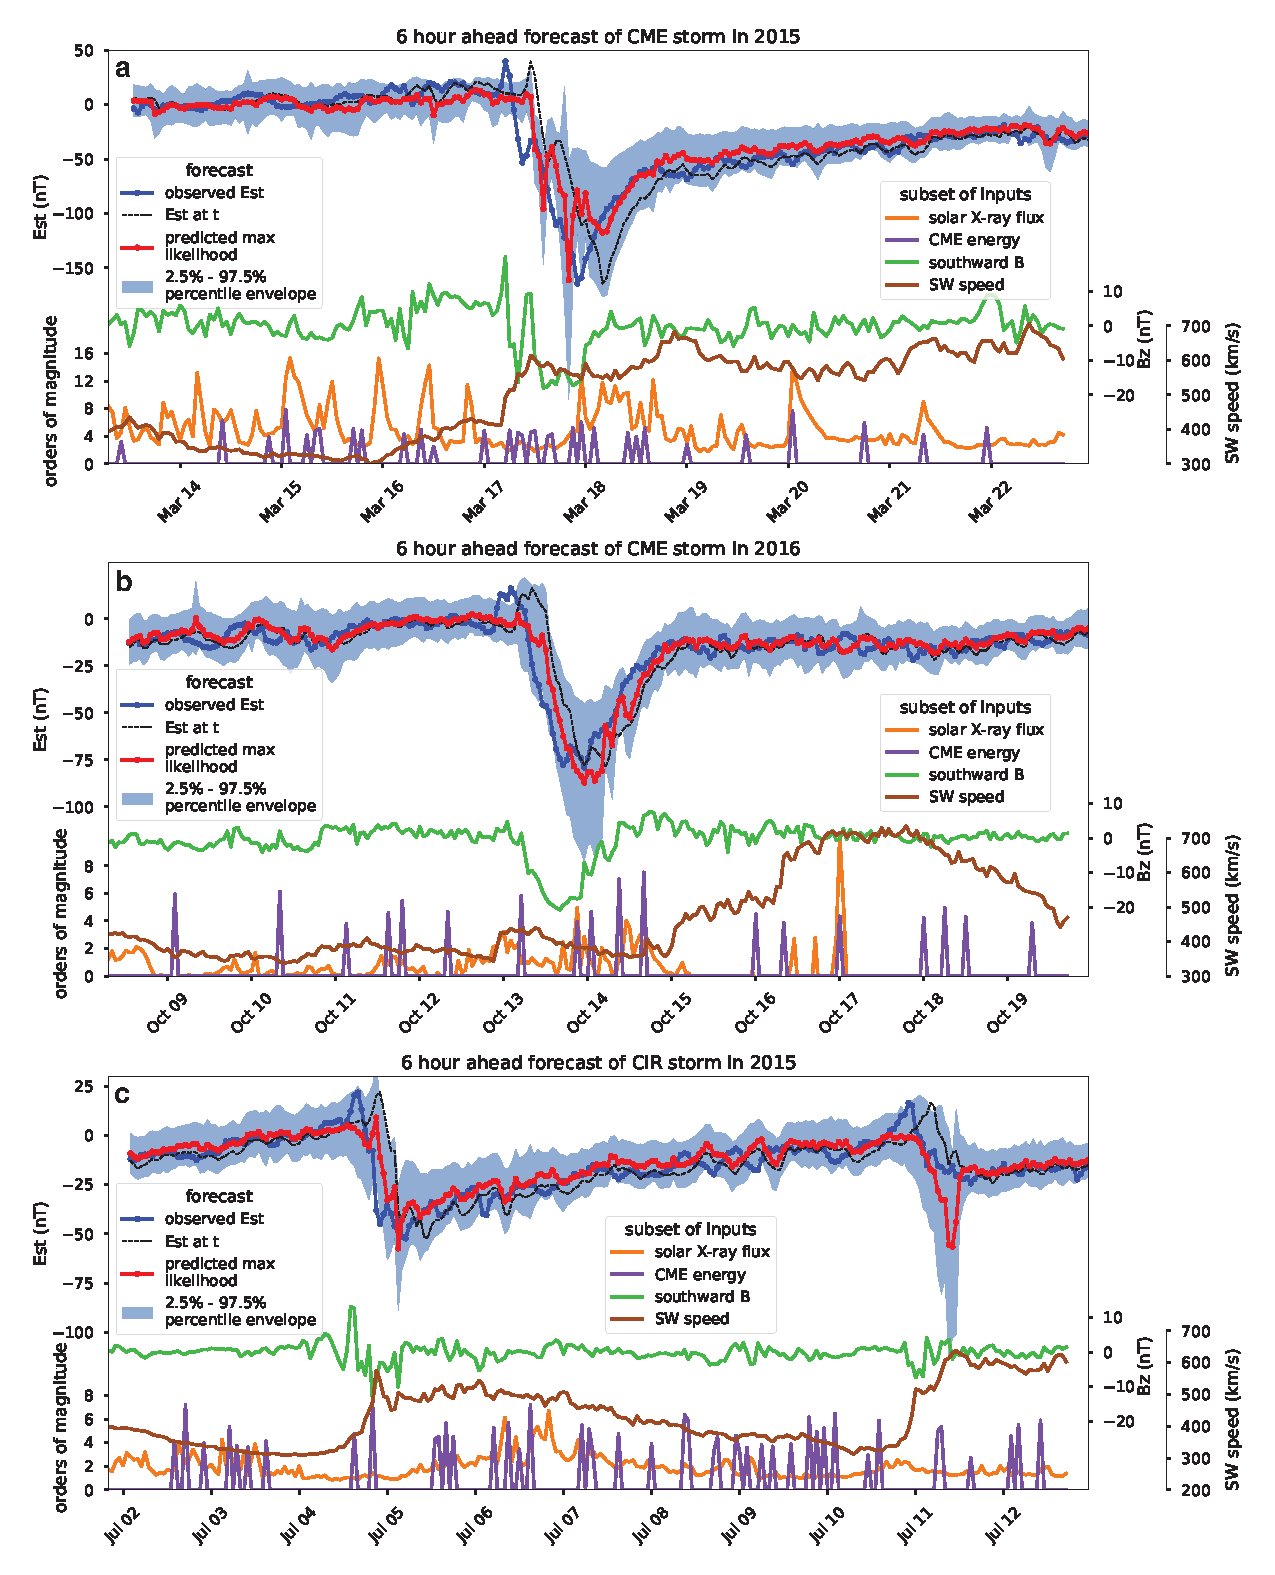
\includegraphics[width=1.0\textwidth]{figures/storms.pdf} 
  \caption{Six-hour-ahead probabilistic forecasts on testing data for two CME storms and one CIR storm, as identified by \cite{Patel2019, Shen2017}. Order of magnitude variability in x-ray flux (long channel is plotted) is exaggerated by ten times. The black dashed line for Est is a persistence forecast. \textbf{(a)} Severe CME geomagnetic storm (min Dst=-222~nT). Large amplitude variability in the southward component of the IMF might be responsible for forecast variability as the storm enters the main phase. \textbf{(b)} Intense CME geomagnetic storm (min Dst=-104~nT). \textbf{(c)} Intense CIR geomagnetic storm (min SYM-H=-87~nT). Order of magnitude variability in x-ray flux here is only exaggerated by five times.}
  \label{fig:storms}
\end{figure}

The first storm, in March of 2015, provides a prototypical example of a geomagnetic storm caused by a magnetic cloud emitted by the mass ejection visible as the spike in CME energy at the beginning of March 15 (Figure~\ref{fig:storms}A, note that the axis is orders of magnitude) \citep{Patel2019}. The energetic mass ejection is associated with a peak in integrated x-ray fluxes, followed two days later by a relatively large geomagnetic storm beginning on March 17. The storm main phase is associated with a sustained southward IMF of roughly -20~nT and roughly doubled solar wind speeds. In this situation, given the clear connection between the mass ejection and the ensuing storm, we would expect a successfully trained network to be able to expand uncertainty in its forecast as conceivable storm arrival times approach, reflecting an understanding of the causal association between activity on the solar disk and geomagnetic storms. Yet, forecast uncertainties only expand when disturbed solar wind reaches the L1 point. At that time, the network becomes aware of the storm arrival and adjusts its output by dropping Est forecasts and increasing forecast uncertainty (Figure~\ref{fig:storms}A). The same is true for the smaller amplitude CME storm of October 13, 2016 in Figure~\ref{fig:storms}B, where forecast uncertainty only grows as soon as the storm arrives at the L1 point. This storm is associated with the CME visible on October 10 \citep{Patel2019}, so the occurrence of other CMEs of similar magnitude (e.g. on October 9 and 11) demonstrates non-uniqueness that illustrates why the network struggles to identify geoeffective solar activity from the provided inputs.

The final storm on July 4, 2015 was chosen because it corresponds to a CIR \citep{Shen2017}, as evidenced by a lack of sustained, southward IMF, a step increase in solar wind velocity, and relatively low amplitude storm-time Est (Figure~\ref{fig:storms}C). The nature of CIR storms differs from those originating from CMEs \citep{Zhang2007}, so we sought to investigate if the forecast for CIR storms differs from that for CME storms. Again, for the storm on July 4, the network is unable to preemptively expand forecast uncertainties in response to information from solar disk, demonstrating that inputs from the L1 point dominate the forecast. On July 11, the network mistakenly forecasts a storm main phase, likely in response to the increased solar wind speed that did not actually generate a substantial main phase.

% forecasting skill
In all cases, \replaced{the six hour ahead forecast fails to capture}{forecasting geomagnetic} storm onset\replaced{, during which the network's forecasts tend to lag observations by the forecast length (thereby more closely tracking the persistence curve) until the storm arrives at the L1 point. At that point, the forecast begins to deviate from persistence as the network knows that a storm is occurring. This inability to predict storm onset indicates that the network is unable to utilize observations from the solar disk for storm arrival, which remains an open challenge.}{is not improved by utilizing observational inputs from the solar disk.} 

\replaced{R}{but r}ecovery is generally well-predicted, and forecasts deviate from persistence, meaning that the network is not just taking the last observed Est value for its next forecast. Unlike previous results, our network is capable of generating meaningful estimates of uncertainty in its forecasts. In all cases, once the network detects the possible onset of a geomagnetic storm, it expands its forecast uncertainty, generally maintaining observed Est values within the 95\% forecast confidence interval and providing reliable multiple hour ahead forecasts (see Supplement Text S5 for one to six hour ahead forecasts). After storm main phases, forecast uncertainties decrease during the generally well-predicted recovery phase. Given that the recovery phase is dictated by the internal dynamics of the ring current decay (and thereby independent of the solar wind state) \citep{Daglis2007}, its predictability is reasonable. Thus, our network exhibits forecast uncertainties that are consistent with where one would anticipate the greatest uncertainty in geomagnetic storm development with information from the L1 point, namely, the storm onset and main phase.

% forecasting skill, conventional metrics
\subsection{\added{Conventional Metrics of Forecast Skill}}

\added{In terms of the conventional forecasting skill assessments (i.e., forecast-observation Pearson correlation coefficients and root-mean-square errors, RMSE's) for one to six hour ahead forecasts, our networks outperform all previous neural network forecasts for all forecasts lengths (Figure~\ref{fig:skill}). However, given that persistence forecasting for Est results in higher correlation coefficients and lower RMSE's than for persistence forecasting of Dst, our improvements should not be compared with previous results for forecasting Dst but with persistence forecasting of Est. When considering all observations, we slightly underperform persistence forecasting of Est in terms of the correlation coefficient, while outperforming in terms of RMSE, which is consistently lower. During storm times, however, our forecasting skill is much better than persistence forecasting in both metrics at all forecasting windows. The networks with both L1 and solar disk inputs always outperform networks with only L1 inputs when evaluated over both quiet and storm times (Figure S9). However, the difference in skill is small, and when considering only storm times, the five to six hour ahead forecasts of networks with only L1 inputs achieve lower RMSE's. These results again indicate that information from the solar disk does not significantly improve storm forecast skill. Finally, for particularly large storms exceeding Est $\leq$ -200~nT, a forecast saturation effect is observed (Figure S9), similar to that that occurs at smaller values with different cost functions (Supplement Text S3). This effect can be partially mitigated by fine-tuning of the cost function to further facilitate the forecasting of rare storms. However, since there is only a handful of such events in the data, this behaviour of the network is natural.}

\begin{figure}[htbp]
  \centering
  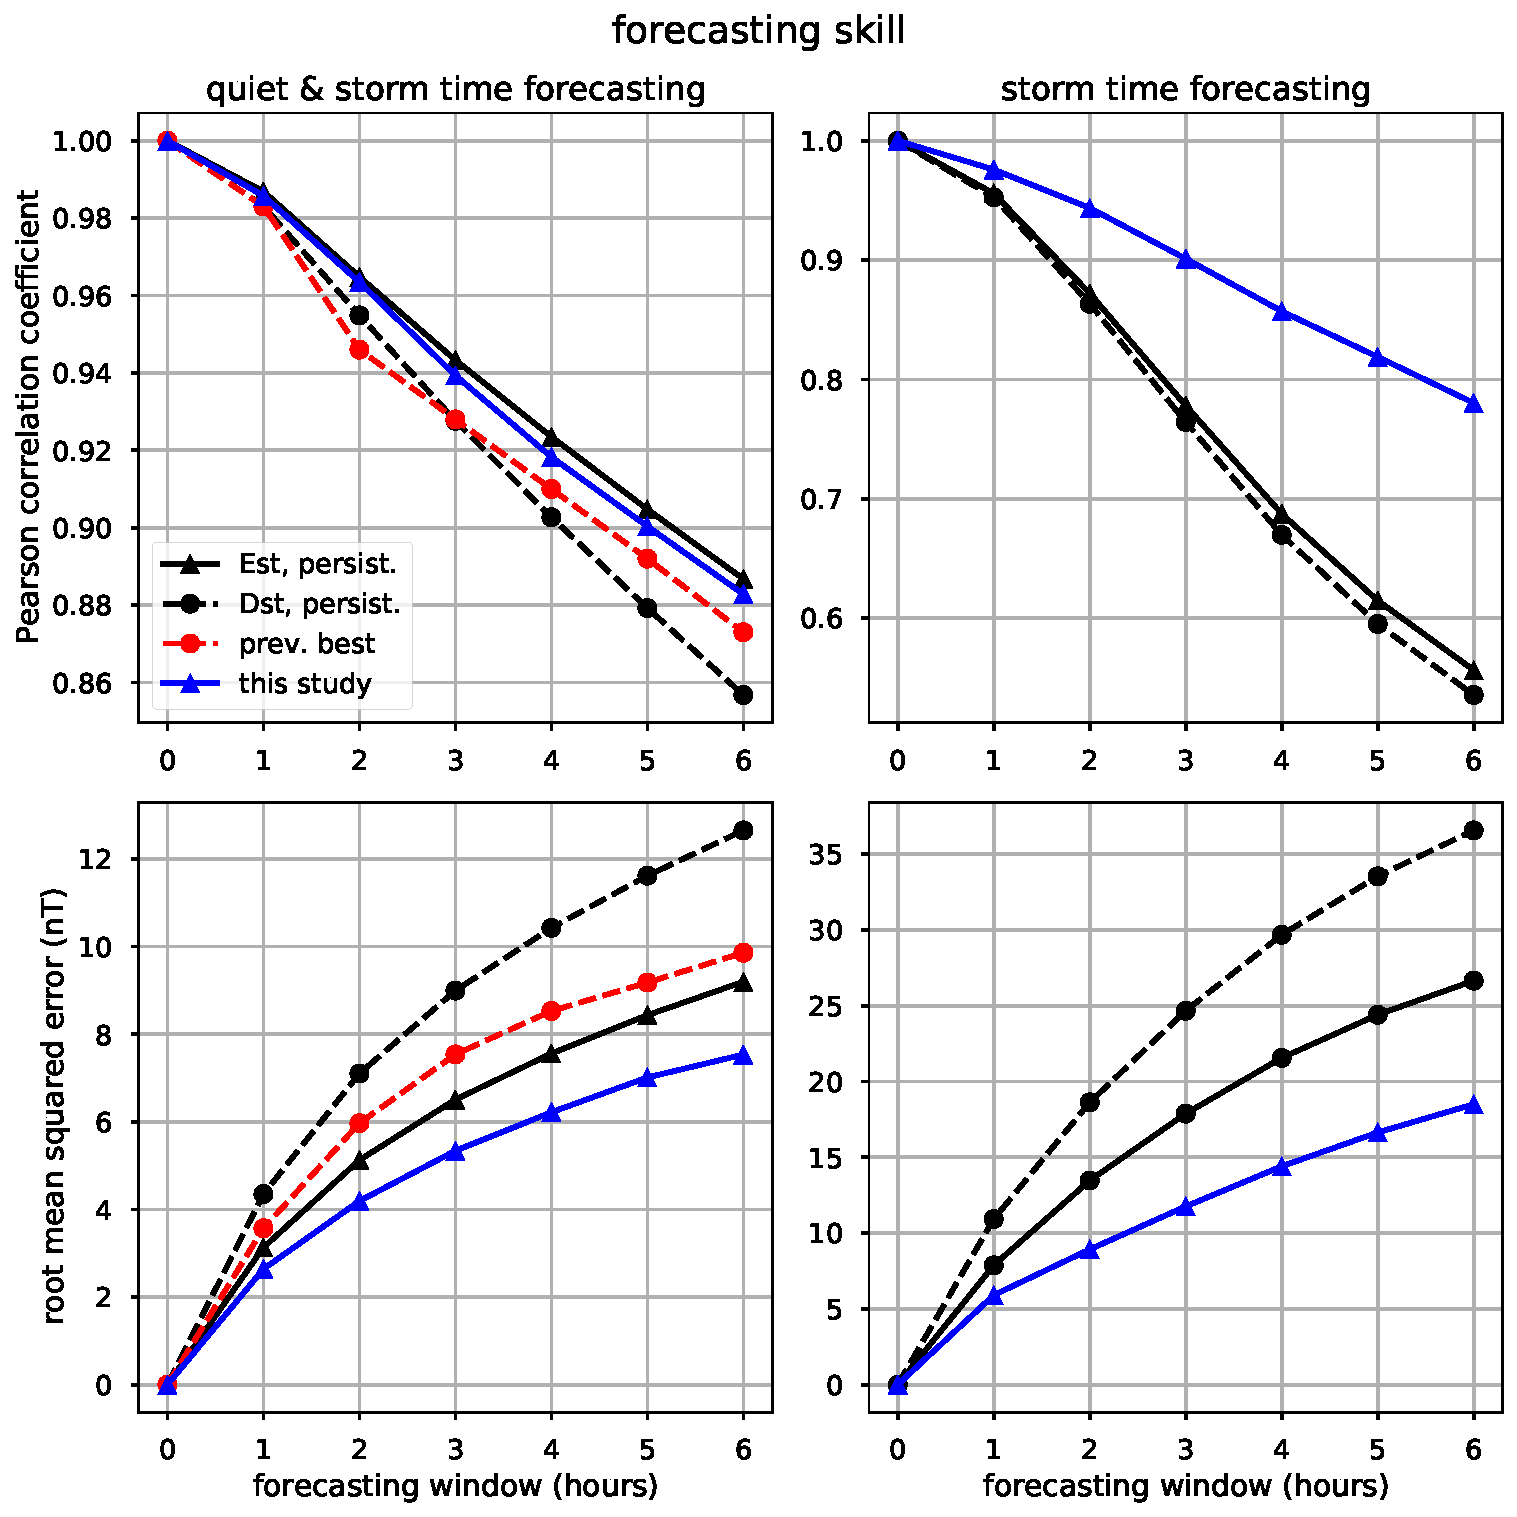
\includegraphics[width=1.0\textwidth]{figures/skill_comparison.pdf} 
  \caption{\added{Conventional metrics of forecasting skill for networks with both solar disk and L1 inputs (see Figure S9 for networks with only L1 inputs). The first row shows the Pearson correlation coefficient between the forecasted Est (mean, for our study) or Dst and the observed Est or Dst. The second row shows the corresponding root mean squared errors. In the columns, we show these quantities for all observations (first column) and only storm-time observations (second column). The black lines show the metrics for persistence forecasts of Est and Dst, and the red line (available only for all observations) shows the best reported performance from NN forecasts (see Table S1 for references).}}
  \label{fig:skill}
\end{figure}


% forecast reliability
\subsection{\added{Forecast Reliability}}

Reliabilities for four different storm thresholds generally overlap with the consistency intervals for each bin, demonstrating that our network generates reliable forecasts (Figure~\ref{fig:reliability}). For threshold of -75 and -100~nT, forecasted exceedance probabilities in the range of 0.7-0.9 tended to slightly underestimate observed exceedance rates, which is consistent with the observation that storm onsets remain difficult to predict exactly.

% adjust wording here
Notably, the regularization of the cost function for a Gaussian output distribution significantly improves forecast reliability. Networks trained with unregularized Gaussian and Gumbel output distributions (Supplement Text S3) are unable move the location parameters of their forecasts during large amplitude storms, preferring instead to expand forecast uncertainty, meaning that peak storm times, while often within the 95\% confidence interval, are only predicted at extremely low exceedance probabilities. This behavior explains why the reliability curves lack data to bin at high forecast probabilities and furthermore why storms are underestimated for lower exceedance probabilities (Figure~\ref{fig:reliability}).

\begin{figure}[htbp]
  \centering
  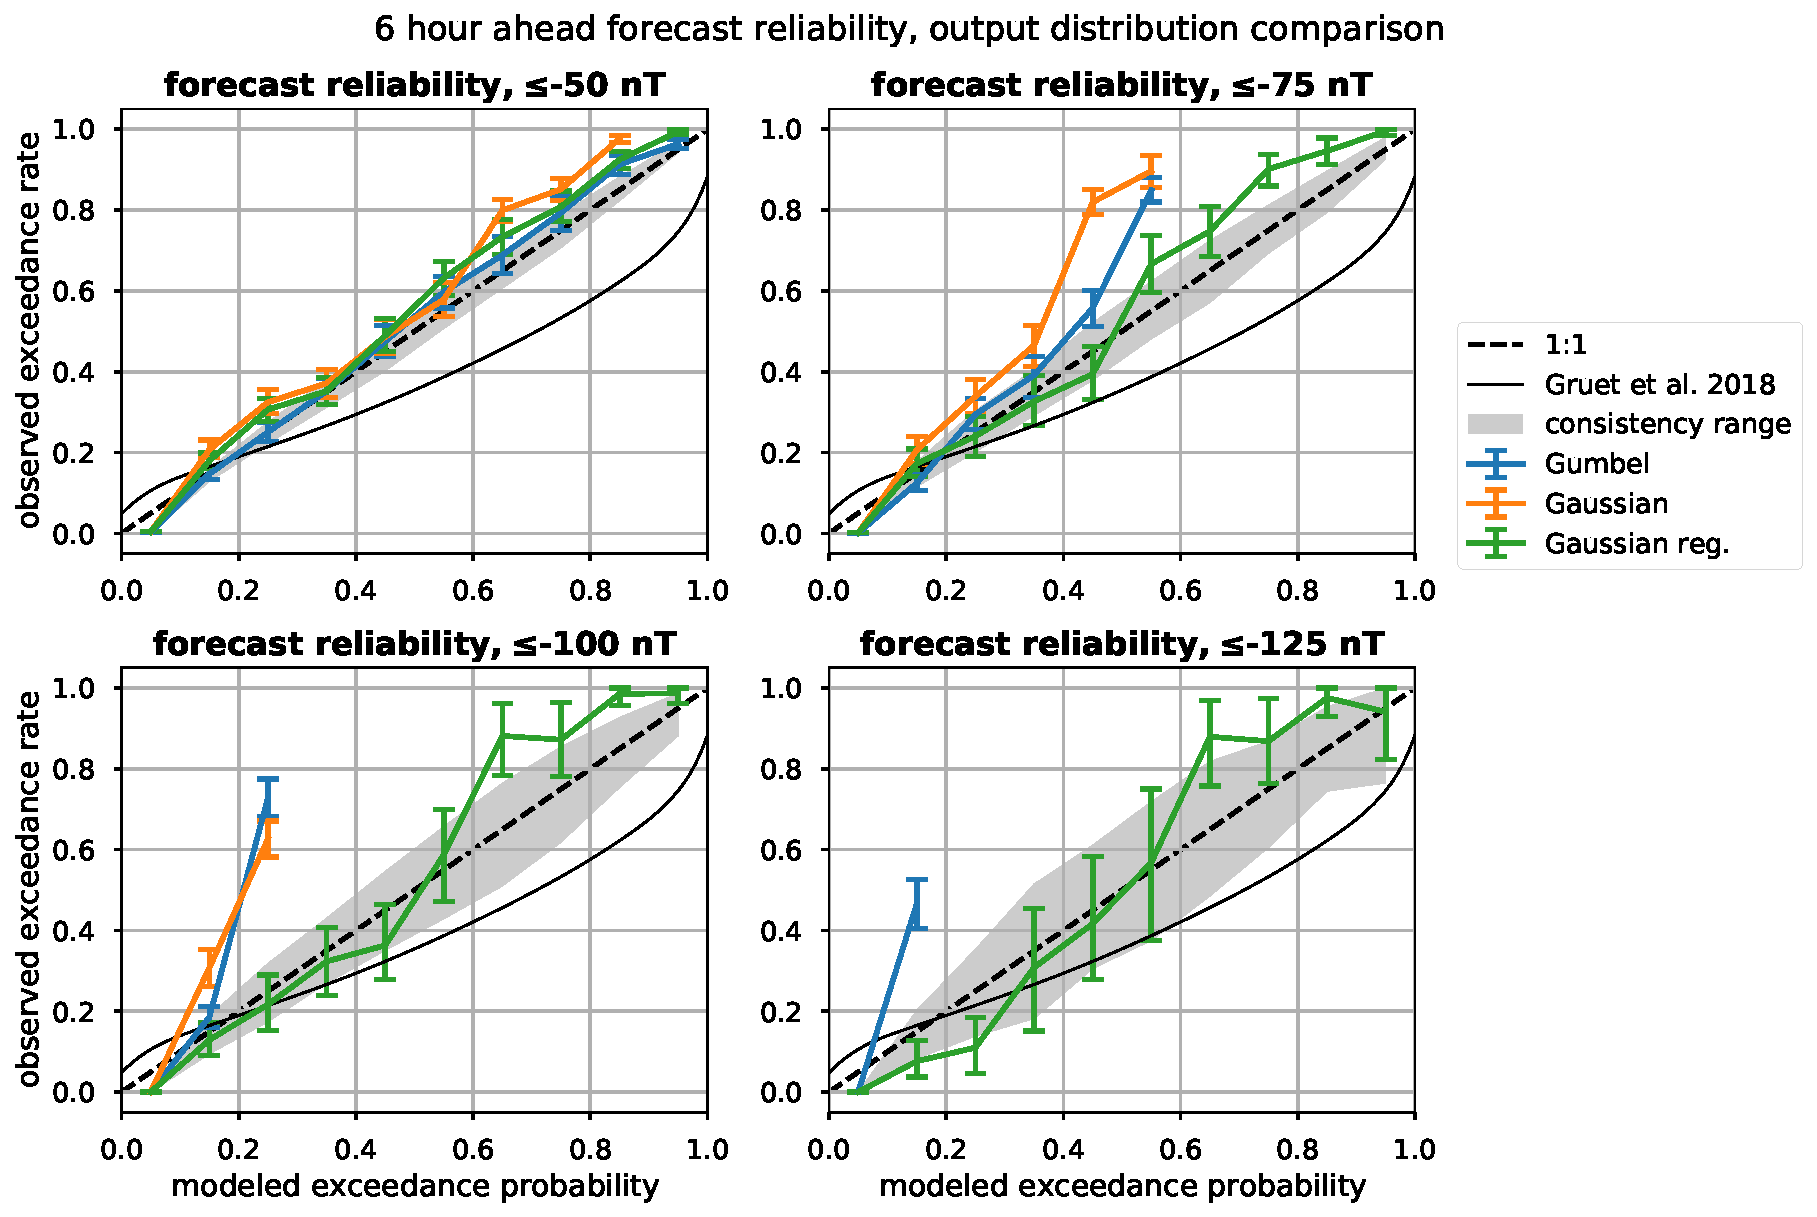
\includegraphics[width=1.0\textwidth]{figures/est_forecast_reliability_distcompare_t+6.pdf} 
  \caption{Reliability curves for the networks with a Gumbel output and cost (blue), Gaussian output and cost (orange), and Gaussian output with regularized cost (green). All curves are for a six hour ahead forecast for four Est thresholds in eleven bins. Exceedance was taken in the negative sense, i.e., taking values less than or equal to the given threshold. Error bars show the 2.5-97.5 percentile range from bootstrapped resampling (number of bootstrapped samples was 1000) within the bins of forecasted exceedance probability. The envelopes show the 2.5-97.5 percentile range from consistency resampling of a perfectly reliable forecast, demonstrating the conceivable range in reliable forecasts given the number of data in each bin \citep{Brocker2007}. The regularized Gaussian network is the most reliable of the three. \added{Also shown is the reliability curve from \cite{Gruet2018} for their six hour ahead Dst forecast, for which the exceedance threshold is unspecified.}}
  \label{fig:reliability}
\end{figure}

While some improvement in forecast reliability for smaller magnitude storms (Est thresholds of -50 and -75~nT) does seem to result from the incorporation of data from the solar disk (Supplement Figure S7), the preceding discussion and the result that forecast behavior does not qualitatively change by adding solar disk inputs (Supplement Text S5) indicates that we are unable to successfully utilize observations from the solar disk to forecast storm arrival and amplitude. This shortcoming suggests that the information necessary for identifying geoeffective solar activity is lacking in the training data, and/or that the network architecture is inadequate for utilizing these data. For instance, the x-ray fluxes are integrated over the entire solar disk, but peaks in these fluxes can often be associated with flare events, which themselves often occur simultaneously with geoeffective mass ejections \citep{Tobiska2013}. Larger, more central flares are associated with larger geomagnetic storms, so adding time series of flare occurrences with locations on the solar disk would complement the input series of x-ray fluxes and CMEs \citep{Tobiska2013}. Futhermore, the CME dataset only includes ejections visible around the rim of the solar disk, while geoeffective ejections occur towards the center. Thus, only centralized ejections that also emit an observable lobe beyond the rim of the solar disk could be reliably associated with geomagnetic storms, potentially rendering the CME database largely irrelevant for the problem of geomagnetic storm forecasting. Finally, integrated solar x-ray flux peaks from flares have been empirically related to solar wind speeds and geomagnetic storm amplitudes, thereby providing a means of learning lag times between solar activity and storm arrivals \citep{Tobiska2013}. However, LSTM networks struggle with learning lag times \citep{Gers2002}, so the network architecture we have utilized is not amenable to this task.  